\subsection{Tenant ages}
\label{sec:application:building_the_model:tenant_ages}

In the tenth step, yet another data field is introduced. In this step, the $.\type{Tenant}$ class is enriched with an $\type{age}$ field and its values. As before, \cref{subsec:library_of_transformations:type_level_transformations:data_fields} is used to introduce the field, while on the instance level, \cref{subsec:library_of_transformations:instance_level_transformations:data_field_values} is used to introduce the values.

The $classtype$ of the new field is $.\type{Tenant}$, as the field will be defined for tenants. The $name$ of the new field is $\type{age}$ and the $fieldtype$ is $\type{int}$. The set of objects of which the value is set is is equal to all tenant objects, so $objects = \{Tenant1, Tenant2, Tenant3, Tenant4, Tenant5\}$. The function for $obids$ returns the existing identifier of each of these objects. The $values$ function is defined as follows:
\begin{align*}
    values = values = \{&(Tenant1, 23), (Tenant2, 24), (Tenant3, 18), \\&(Tenant4, 24), (Tenant5, 19)\}
\end{align*}

The following model is obtained:

\LTXtable{\textwidth}{tex/06_application/02_building_the_model/tables/10_tenant_ages.tex}

\begin{figure}[p]
    \centering
    \begin{subfigure}{0.98\textwidth}
        \centering
        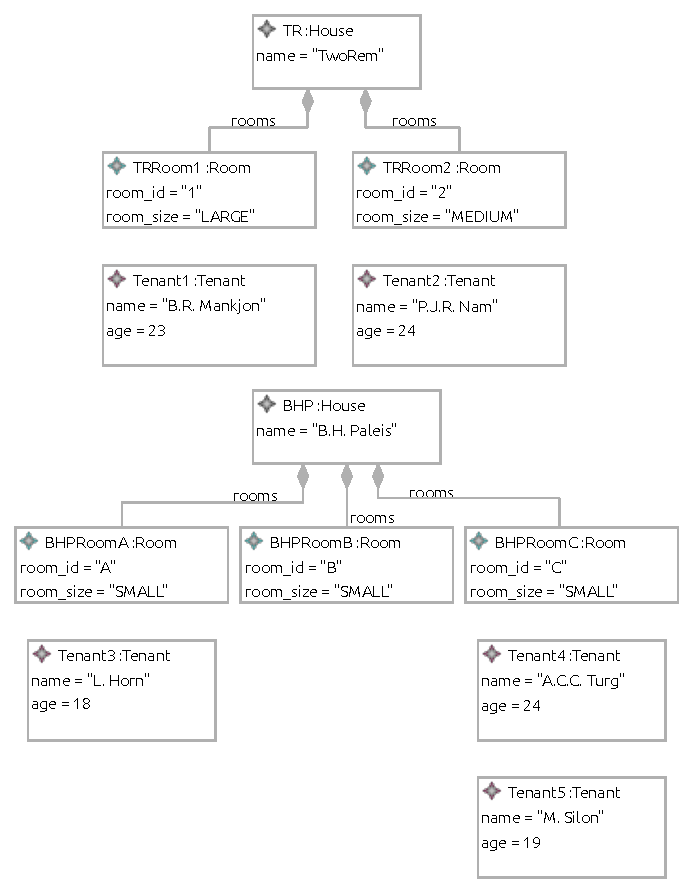
\includegraphics{images/06_application/instance_model/step10.pdf}
        \caption{Instance Model $Im_{10}$}
        \label{fig:application:building_the_model:tenant_ages:ecore:instance_model}
    \end{subfigure}
    \\
    \begin{subfigure}{0.98\textwidth}
        \centering
        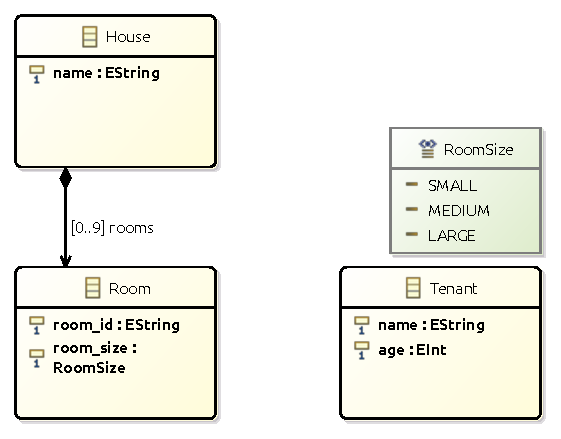
\includegraphics{images/06_application/type_model/step10.pdf}
        \caption{Type Model $Tm_{10}$}
        \label{fig:application:building_the_model:tenant_ages:ecore:type_model}
    \end{subfigure}
    \caption{The Ecore model after step 10}
    \label{fig:application:building_the_model:tenant_ages:ecore}
\end{figure}

\begin{figure}[p]
    \centering
    \begin{subfigure}{0.98\textwidth}
        \centering
        % To use this figure in your LaTeX document
% import the package groove/resources/groove2tikz.sty
%
\begin{tikzpicture}[scale=\tikzscale,name prefix=step10-]
\node[type_node] (n0) at (0.740, -0.400) {\ml{\textbf{House}\\name: \textbf{string}}};
\node[type_node] (n1) at (0.730, -1.585) {\ml{\textbf{Room}\\room\_id: \textbf{string}}};
\node[type_node] (n2) at (2.380, -0.560) {\ml{\textbf{RoomSize}\\\textit{LARGE}\\\textit{MEDIUM}\\\textit{SMALL}}};
\node[type_node] (n3) at (2.500, -1.590) {\ml{\textbf{Tenant}\\age: \textbf{int}\\name: \textbf{string}}};

\path[basic_edge, composite](n0.south -| 0.730, -1.585) -- node[lab] {\ml{rooms}} (n1) ;
\path[basic_edge] (n1)  -- node[lab] {\ml{room\_size}} (n2) ;
\end{tikzpicture}

        \caption{Instance Graph $IG_{10}$}
        \label{fig:application:building_the_model:tenant_ages:groove:instance_graph}
    \end{subfigure}
    \\
    \begin{subfigure}{0.98\textwidth}
        \centering
        % To use this figure in your LaTeX document
% import the package groove/resources/groove2tikz.sty
%
\begin{tikzpicture}[scale=\tikzscale,name prefix=step10-]
\node[type_node] (n0) at (0.740, -0.400) {\ml{\textbf{House}\\name: \textbf{string}}};
\node[type_node] (n1) at (0.730, -1.585) {\ml{\textbf{Room}\\room\_id: \textbf{string}}};
\node[type_node] (n2) at (2.380, -0.560) {\ml{\textbf{RoomSize}\\\textit{LARGE}\\\textit{MEDIUM}\\\textit{SMALL}}};
\node[type_node] (n3) at (2.500, -1.590) {\ml{\textbf{Tenant}\\age: \textbf{int}\\name: \textbf{string}}};

\path[basic_edge, composite](n0.south -| 0.730, -1.585) -- node[lab] {\ml{rooms}} (n1) ;
\path[basic_edge] (n1)  -- node[lab] {\ml{room\_size}} (n2) ;
\end{tikzpicture}

        \caption{Type Graph $TG_{10}$}
        \label{fig:application:building_the_model:tenant_ages:groove:type_graph}
    \end{subfigure}
    \caption{The GROOVE graphs after step 10}
    \label{fig:application:building_the_model:tenant_ages:groove}
\end{figure}

A visual representation of $Tm_{10}$ and $Im_{10}$ can be found in \cref{fig:application:building_the_model:tenant_ages:ecore}. Similarly, a visual representation of $TG_{10}$ and $IG_{10}$ can be found in \cref{fig:application:building_the_model:tenant_ages:groove}. Please note that because of the definitions of $f_{10}(Im_{10})$ and $f'_{10}(IG_{10})$, we have that $f_{10}(Im_{10}) = IG_{10}$ and $f'_{10}(IG_{10}) = Im_{10}$. Furthermore, $f_{10}(Im_{10})$ and $f'_{10}(IG_{10})$ are valid mapping functions themselves, such that they can be combined with another mapping function in the next step.

The introduction of age for the tenant shows that the data field transformation can also be applied with another type than $\type{string}$. The visualisation shows the different ages for the different tenants visually.

\afterpage{\FloatBarrier}